\chapter{Exponential Expressions}
\label{ch:expoexpr}

\chapquote{Still need to find a quote that works for this chapter. In the meantime, we have this.}{Author\\Description of author}

%\begin{quote}
%Still need to find a quote that works for this chapter. In the meantime, we have this.
%\par \hfill --- Author, description of author
%\end{quote}

Every chapter should have a lead paragraph -- even just a short one -- that appears before the first heading. This is a placeholder paragraph which will at some point be replaces by actual content.

% % % % % % % % % % % % % % % % % % % % % % % % % % % % % % % % % % % % % % % % 
\section{Fundamentals of Exponents}
\label{sec:exposimpform}

%\begin{boxedexplore}[Startup Exploration: TODO]
%TODO
%\end{boxedexplore}

%When we talk about exponents and exponential expressions, we're talking about expressions of the form: $a^b$. This is read ``$a$ to the power of $b$'' or ``$a$ to the $b^{\text{th}}$ power''. In such an expression, $a$ is called the \textit{base} and $b$ is called the \textit{exponent}. Since $a$ is the base, we call the whole thing a \textit{power of $a$}.
%
%One interpretation of this expression, as we have seen, is a repeated multiplication:
%\[a^b = \underbrace{a \cdot a \cdot a \cdot \dotsm \cdot a}_{\text{$b$ times}}\]
%
%
%There are three ways to write a quantity:
%
%Expanded Form, Exponent Form, and Standard Form. Exponential form is the ``short'' way of writing Expanded Form. Technically, the expanded form and the exponent form are linked by the definition of a power ($a^n = a*a*a...*a$, where there are n factors). Standard Form is like the ``answer.'' Not every power will have a standard form, only the ones with numbers for bases.
%
%Expanded Form: 12*12*12*12, Q*Q*Q*Q*Q*Q
%
%Exponent Form: $12^4$, $Q^6$, $2^x$
%
%Standard Form:  20,736
%
%Note: There are many things in math that are called ``standard form''. Now we have two, standard form of a number and standard form for a linear equation. You are going to have to look at context clues to determine which one you need.
%
%\subsection{Reminder: One of the Trickiest Concepts in Algebra 1}
%
%We first saw this tricky little item back in \cref{ch:numbers}, and haven't really had to deal with it again until now. Recall the difference between the following three expressions:
%\[(-2)^4 \qquad\text{and}\qquad -2^4\]
%If we write these out in expanded form we have \[(-2)^4 = (-2)(-2)(-2)(-2) = 16.\] On the other hand, \[−2^4 = −2\cdot2\cdot2\cdot2 = -16.\] Be careful not to jump to conclusions, though! Compare these two:
%\[-2^3=-2\cdot2\cdot2= -8 \text{\qquad and \qquad} (−2)^3 = (-2)(-2)(-2) = -8\]
%Whenever we are asked to simplify an exponential expression, a good habit of mind is to ask ourselves, ``What, exactly, does the exponent apply to?''

\section{Simplified Algebraic Expressions: Exponents Edition}

In earlier chapters we learned properties that could be used to simplify linear expressions. The criteria we learned in \cref{ch:equations} for ``simplified algebraic expressions'' still apply, but now that we are dealing with exponents, there are a few new criteria that we need to add. We will summarize the criteria here and then learn the details over the next few sections.

\begin{boxedcriteria}[Simplified Exponential Expressions]
An exponential expression is considered completely simplified if\ldots
\begin{enumerate}
	\item It contains only positive exponents
	\item Bases appear at most once per term
	\item Powers with a numeric base are written in standard form (if that's reasonable)
	\item It contains no explicit grouping symbols
\end{enumerate}
\end{boxedcriteria}

Criteria \#1 asks for only positive exponents. In \cref{sec:exponegative}, we saw how to use the reciprocal to rewrite a negative exponent using a positive exponents. We'll see more about negative exponents in \cref{sec:expoquotient}.

Criteria \#2 prohibits a term to be written in the form $x^2 \cdot x^3$, since this is a term that has the same base ($x$) appearing twice. In a way, we're looking for a kind of ``combining like terms'' that will allow us to write this as $x$ raised to a single exponent. Properties of this kind will be the main focus in this chapter.

Criteria \#3 asks us to evaluate expressions like $2^3$ and write 8 instead\ldots\ if that's reasonable. We have already seen that exponential expressions can yield some enormous numbers, so it's better to write $6^{12}$ than $2\,176\,782\,336$. Use your best judgement here: a number that's larger than, say, five digits should probably be left in exponential form. It's also best to continue our convention of using simplified improper fractions instead of decimals.

Criteria \#4 is already in effect: explicit grouping symbols have been banned from simplified algebraic expressions since \cref{ch:equations}. We mention it again here because some special care is required when it comes to eliminating groupers that are tangled up with exponents.

\subsubsection{Remember: Order of Operations}

The expression $2 \cdot 3^x$ is completely simplified. We might be tempted to write $6^x$, but this would be \evilandwrong. Since exponents must be evaluated before multiplication, it is impossible to fully evaluate this expression, We don't know what $x$ is, and so it is impossible to resolve the expression $3^x$, and so we cannot do the multiplication. So, we stop here.

\subsubsection{Exponent Properties}

In the next few sections we will derive the properies for simplifying exponential expressions and achieveing simplified exponential form.\footnote{These aren't all of the definitions and properties for exponents, but they are the key ones we need for now. We will learn a few more tools in later chapters when we look at quadratics, polynomials, and radicals. There are also a few saved for algebra 2, when we will see non-integer exponents and logarithms.} With each new property, work out the initial examples and think about how to state a general simplification rule.

% % % % % % % % % % % % % % % % % % % % % % % % % % % % % % % % % % % % % % % % 
\section{Product Properties}
\label{sec:expoproduct}

\subsection{The Product Rule}

\begin{boxedexplore}[Startup Exploration: Derivation \#1]
Use expanded form to write each of the expressions below as a single base raised to a singe exponent.
\[x^4 \cdot x^3 \qquad\text{and}\qquad z^5 \cdot z^8\]
Make a conjecture about a general rule for simplifications of this type.
\end{boxedexplore}

This shortcut is called the product rule, since it applies to the situation in which we are finding the product of two exponential expressions with the same base.

We can write the first example out in expanded form, and then rewrite the long string of $x$'s under a single exponent:
\[{\color{red}x^4} \cdot {\color{blue}x^3} = {\color{red}x \cdot x \cdot x \cdot x} \cdot {\color{blue}x \cdot x \cdot x} = x^7\]
The same goes for the $z$'s in the second expression:
\[{\color{red}z^5} \cdot {\color{blue}z^8} = {\color{red}z \cdot z \cdot z \cdot z \cdot z} \cdot {\color{blue}z \cdot z \cdot z \cdot z \cdot z \cdot z \cdot z \cdot z} = z^{13}\]

The new exponent will be the sum of the original exponents!

\begin{boxeddef}[Product Rule of Exponents]
For any nonzero real number $a$ and any integers $m$ and $n$, \[a^m \cdot a^n = a^{m+n}.\]
\end{boxeddef}

The intuition behind this rule is that $a^m \cdot a^n$ means we have $m$ factors of $a$ multiplied by $n$ factors of $a$, and so we have $m+n$ factors of $a$ in all. That means $a^{m+n}$. This is pretty straightforward! There's really no need to ``memorize'' this rule. We can always re-derive it if we forget exactly how it works.

\begin{boxedex}
Simplify $3b^2 \cdot 4b^5.$

\exsoln\ In this example, we will need to use the commutative property of multiplication to move the coefficients together and the variable parts together. In other words: \[3b^2 \cdot 4b^5 = 3\cdot4\cdot b^2 \cdot b^5 = 12b^{2+5} = 12b^7.\]
\end{boxedex}


\subsection{The Power Rule}

\begin{boxedexplore}[Startup Exploration: Derivation \#2]
Use expanded form to write each of the expressions below as a single base raised to a singe exponent.
\[(x^3)^4 \qquad\text{and}\qquad (z^5)^8\]
Make a conjecture about a general rule for simplifications of this type.
\end{boxedexplore}

This simplification is called the power rule, since it applies to situations in which we have a power which is itself being raised to a power.

Writing the first expression in expanded form gives us a product. From there we can apply the product rule that we learned in the last section:
\[(x^3)^4 = x^3 \cdot x^3 \cdot x^3 \cdot x^3 = x^{3+3+3+3} = x^{4\cdot3} = x^{12}\]
Notice that we get a repeated addition in the exponent, which we can rewrite as a multiplication. In the second expression, we have:
\[(z^5)^8 = z^5 \cdot z^5 \cdot z^5 \cdot z^5 \cdot z^5 \cdot z^5 \cdot z^5 \cdot z^5 = z^{8\cdot5} = z^{40}\]

The new exponent is the product of the original exponents!

\begin{boxeddef}[Power Rule of Exponents]
For any nonzero real number $a$ and any integers $m$ and $n$, \[(a^m)^n = a^{n \cdot m}\]
\end{boxeddef}

In this case, the intuition is that the outermost exponent means we will multiply together $n$ factors of $a^m$. Since each of those factors has $m$ factors of $a$, we have ``$n$ groups of $m$ factors of $a$'' in all, which is another way of saying $n \cdot m$ factors of $a$.

\begin{boxedex}
---
\end{boxedex}


\subsection{Product to a Power}

\begin{boxedexplore}[Startup Exploration: Derivation \#3]
Use expanded form to write each of the expressions below without parentheses.
\[(xy)^4 \qquad\text{and}\qquad (abc)^8\]
Make a conjecture about a general rule for simplifications of this type.
\end{boxedexplore}

In this case, we are taking the power of a product so we call this shortcut ``power of a product'' or ``product to a power''. We can write out the first expression in expanded form, and then use the commutative property to rearrange the factors:
\[(xy)^4 = (xy)(xy)(xy)(xy) = xy\,xy\,xy\,xy = xxxx\,yyyy = x^4y^4\]
The second example works just the same way:
\[
\begin{aligned}(abc)^8 &= (abc)(abc)(abc)(abc)(abc)(abc)(abc)(abc)
\\ &= abc\,abc\,abc\,abc\,abc\,abc\,abc\,abc
\\ &= aaaaaaaa\,bbbbbbbb\,cccccccc
\\ &= a^8b^8c^8
\end{aligned}\]

We can remove the parentheses by attaching the exponent to each of the factors inside!

\begin{boxeddef}[Product to a Power Rule]
For any nonzero real numbers $a$ and $b$ and any integer $m$, \[(ab)^m = a^m b^m\]
\end{boxeddef}

The idea is that the exponent gives us $m$ copies of the product, which means $m$ copies of each of the factors in that product. The commutative property of multiplication allows us to move these factors around and regroup them.

Note that the thing in the parentheses is a product, \textit{not a sum}. We'll learn how to handle sums raised to powers, for example $(x+y)^2$, in \cref{sec:exposumstopowers}.

\begin{boxedex}
---
\end{boxedex}


% % % % % % % % % % % % % % % % % % % % % % % % % % % % % % % % % % % % % % % % 
\section{Quotient Properties} 
\label{sec:expoquotient}

The rules in the last section were all based on multiplication. We'll look at some division-related laws, which behave in a very similar way (since multiplication and division are inverse operations). We pull these rules out into their own section since they bring us into closer contact with negative exponents, which take some getting used to.

\subsection{Simplifying Negative Exponents}

\begin{boxedexplore}[Startup Exploration: Derivation \#4]
Use the definition of a negative exponent to write each of the expressions using only positive exponents.
\[\frac{a^{-2}}{b} \qquad\text{and}\qquad \frac{2x^3y^{-2}}{m^{-5}q^2}\]
Make a conjecture about a general rule for simplifications of this type.
\end{boxedexplore}

We'll use the definition of negative exponents to work these out, but sometimes that can involve numerous steps. For example in the first expression, we have:
\[\frac{a^{-2}}{~b~} = \frac{\frac{1}{a^2}}{~b~} = \frac{1}{a^2}\div{b} = \frac{1}{a^2}\cdot\frac{1}{b} = \frac{1}{a^2b}\]
After going through all of that work, we simply end up with $a^2$ in the denominator. In the second example, we can see that the 2, the $x^3$, and the $q^2$ have positive exponents already and are going to stay right where they are. Let's extract the expressions with negative exponents and treat those separately:
\[\frac{2x^3{\color{blue}y^{-2}}}{{\color{red}m^{-5}}q^2}
= \frac{2x^3}{q^2}\cdot{\color{blue}\frac{y^{-2}}{1}}\cdot{\color{red}\frac{1}{m^{-5}}}
= \frac{2x^3}{q^2}\cdot{\color{blue}\frac{1}{y^2}}\cdot{\color{red}\frac{m^5}{1}}
= \frac{2x^3{\color{red}m^5}}{q^2{\color{blue}y^2}}\]

When we see a negative exponent, we can move that base to the other part of the fraction and change the sign of the exponent.

\subsubsection{Beware of the Headless Fraction}

We may write a number without a denominator. The number 41, for example, has no denominator --- or rather, it has a phantom 1 in the denominator which we don't write unless we need to.

We cannot write a number without a numerator. For example, if we are asked to simplify the expression $g^-6$, we can use the shortcut and put $g^6$ in the other part of the fraction, but now we have an empty numerator\ldots \[g^{-6} = 
\begin{array}{cc}~~&\longleftarrow\text{ what goes here?}
\\\cline{1-1}
g^6 & ~~\end{array}\]
We can't leave the numerator empty because then we don't have a number that makes sense. ``Empty numerator'' might imply ``numerator = 0'', but that would make the whole fraction equal to 0, which would be wrong: if $g\neq0$, then $\frac{1}{g} \neq 0$.

It must be that the numerator is 1. Indeed this makes sense, for we can introduce a phantom 1 before we apply the shortcut:
\[g^{-6} = {\color{violet}1} \cdot g^{-6} = \frac{{\color{violet}1}}{g^6}\]

Notice that in the first example of derivation \#4, we filled the empty numerator with 1, just as we did here.


\subsection{Quotient Rule}

\begin{boxedexplore}[Startup Exploration: Derivation \#5]
Use expanded form to write each of the expressions below as a single base raised to a singe exponent.
\[\frac{m^6}{m^2} \qquad\text{and}\qquad \frac{z^5}{z^8}\]
Make a conjecture about a general rule for simplifications of this type.
\end{boxedexplore}

This simplification is called the quotient rule, since it applies when we are finding the quotient of two exponential expressions with the same base.

When we write out the first expression in expanded form, we have some common factors of $x$ which ``cancel'' from the numerator and denominator.
\[\frac{m^6}{m^2} = \frac{m\,m\,m\,m\,m\,m}{m\,m} = \frac{m\,m\,m\,m\,\cancel{m}\,\cancel{m}}{\cancel{m}\,\cancel{m}} = \frac{m\,m\,m\,m}{1} = m^4\]
Here, we replace the empty denominator with a soon-to-be phantom 1, which promptly vanishes. In the second example, the leftovers are in the denominator.
\[\frac{z^5}{z^8} = \frac{z\,z\,z\,z\,z}{z\,z\,z\,z\,z\,z\,z\,z} = \frac{\bcancel{z}\,\bcancel{z}\,\bcancel{z}\,\bcancel{z}\,\bcancel{z}}{\bcancel{z}\,\bcancel{z}\,\bcancel{z}\,\bcancel{z}\,\bcancel{z}\,z\,z\,z} = \frac{1}{z^3} = z^{-3}\]

The new exponent is the difference of the original exponents: numerator minus denominator!

\begin{boxeddef}[Quotient Rule]
For any nonzero real number $a$ and any integers $m$ and $n$, \[\frac{a^m}{a^n} = a^{m-n}\]
\end{boxeddef}

The intuition here is that when we have a quotient involving two expressions with the same base, there are going to be common factors in the numerator and denominator. Some of these will ``cancel'', and in fact either the whole numerator or the whole denominator (or both!) will be reduced simply to the number 1.

Since multiplication and division are inverse operations, this rule can be seen as a version of the product rule if we allow negative exponents:
\[\frac{a^m}{a^n} = a^m \cdot a^{-n} = a^{m+\umin n} = a^{m-n}\]

This rule also helps us to understand the zero exponent. We know that anything divided by itself is 1, and so for instance: \[\frac{a^m}{a^m} = 1 \qquad\text{since a number divided by itself is 1}\]
If we interpret this using the quotient rule, we have: \[\frac{a^m}{a^m} = a^{m-m} = a^0 \qquad\text{application of the quotient rule}\]
This means we have two different interpretations of the same quantity, and so these two interpretations must be equal. In other words, it must be that: \[a^0 = 1.\]


\subsection{Quotient to a Power}

\begin{boxedexplore}[Startup Exploration: Derivation \#6]
Use expanded form to write each of the expressions below without parentheses.
\[\left(\frac{x}{y}\right)^2 \qquad\text{and}\qquad \left(\frac{ab}{c}\right)^7\]
Make a conjecture about a general rule for simplifications of this type.
\end{boxedexplore}

By now, you may be getting the hang of these simplification properties! In this case, we have
\[\left(\frac{x}{y}\right)^2 = \left(\frac{x}{y}\right)\left(\frac{x}{y}\right) = \frac{x\cdot x}{y\cdot y} = \frac{x^2}{y^2}\]
The second example is longer, but works the same:
\[\begin{aligned}
\left(\frac{ab}{c}\right)^7
&= \left(\frac{ab}{c}\right)\left(\frac{ab}{c}\right)\left(\frac{ab}{c}\right)\left(\frac{ab}{c}\right)\left(\frac{ab}{c}\right)\left(\frac{ab}{c}\right)\left(\frac{ab}{c}\right)
\\[1ex]&= \frac{ab\,ab\,ab\,ab\,ab\,ab\,ab}{c\,c\,c\,c\,c\,c\,c}
\\[1ex]&= \frac{(ab)^7}{c^7}
\\[1ex]&= \frac{a^7b^7}{c^7}
\end{aligned}\]

In general, when we have a quotient raised to a power, we can apply the exponent to both the numerator and denominator. To eliminate the parentheses entirely in the second example, we had to use the power of a product property to simplify the numerator.

\begin{boxeddef}[Quotient to a Power Rule]
For any nonzero real numbers $a$ and $b$ and any integer $m$, \[\left(\frac{a}{b}\right)^m = \frac{a^m}{b^m}\]
\end{boxeddef}

The exponent means that we have $m$ copies of the fraction $\frac{a}{b}$ which, when we multiply, become a single fraction with $m$ copies of $a$ in the numerator and $m$ copies of $b$ in the denominator.

\subsection{Combo Problems}

The second example in derivation \#6 required us first to simplify the power of a quotient, and then the power of a product. Smashup problems like this require some careful dissection. Consider the following nasty-looking expression
\[\frac{(5x^3)(3x^{-2})}{30x^{12}}.\]
With a monster like this, it is sometimes hard to know how to begin. A good strategy is to proceed one step at a time, carefully applying the properties from this section to try and make this slightly simpler with each step.

For instance, we might start by multiplying in the numerator. We'll have a coefficient ($5\cdot3 = 15$), and we'll use the product property to multiply the variables ($x^3 \cdot x^{-2} = x^{3+\umin2} = x^1$). This gives us:
\[\frac{(5x^3)(3x^{-2})}{30x^{12}} = \frac{15x}{30x^{12}}.\]

Now, we'll need the quotient property to simplify the variables. The coefficients also share a common factor of 15. This will eliminate the numerator entirely!
\[\frac{(5x^3)(3x^{-2})}{30x^{12}} = \frac{15x}{30x^{12}} = \frac{1}{2x^{11}}.\]

That final answer might not look all that ``simple'', but it meets the requirements of a simplified exponential expression, and so we're done. Try the following examples, and then study the solutions carefully.

\begin{boxedex}
Simplify each of the following.
\[\left(\frac{x^3y^{-2}}{x^{-1}y^5}\right)^3 \qquad\text{and}\qquad \frac{8x^2y}{y^2}\div\frac{16xy^2}{(4y^2)^2}\]

\exsoln\ We recommend simplifying what's inside those parentheses before dealing with the outermost exponent. To simplify the insides, we'll need to move some negative exponents, and then apply the product property.
\[\left(\frac{x^3y^{-2}}{x^{-1}y^5}\right)^3
= \left(\frac{x^3x^{1}}{y^5y^2}\right)^3
= \left(\frac{x^{3+1}}{y^{5+2}}\right)^3
= \left(\frac{x^4}{y^7}\right)^3
= \frac{x^{4\cdot3}}{y^{7\cdot3}}
= \frac{x^{12}}{y^{21}}
\]
The last thing we did was apply the power of a quotient to get our final answer. To tackle the second problem, recall that division is like multiplication by the reciprocal. 
\[\frac{8x^2y}{y^2}\div\frac{16xy^2}{(4y^2)^2} = \frac{8x^2y}{y^2}\cdot\frac{(4y^2)^2}{16xy^2}\]
Then, before we can apply any of the product properties, we need to fix the product of a power, which will in turn require the power property: $(4y^2)^2 = 4^2 \cdot (y^2)^2 = 16 y^{2\cdot2} = 16y^4$. From here, we can simplify the individual fractions, then apply the product property to multiply them, and then apply the quotient property (again) to simplify the result.
\[\begin{aligned}
\frac{8x^2y}{y^2}\div\frac{16xy^2}{(4y^2)^2}
&= \frac{8x^2y}{y^2}\cdot\frac{(4y^2)^2}{16xy^2}
\\[1ex]&= \frac{8x^2y}{y^2}\cdot\frac{16y^4}{16xy^2}
\\[1ex]&= \frac{8x^2}{y}\cdot\frac{y^2}{x}
\\[1ex]&= \frac{8x^2y^2}{yx}
\\[1ex]&= 8xy
\end{aligned}\]
Some of the simplification steps we took above could have been completed in a different order. There are multiple paths to the most simplified form!
\end{boxedex}


% % % % % % % % % % % % % % % % % % % % % % % % % % % % % % % % % % % % % % % % 
\section{Raising Sums to Powers}
\label{sec:exposumstopowers}

\begin{boxedexplore}[Startup Exploration: Check This Work!]
The following is a very common error: \[(a+b)^2 = a^2 + b^2 \qquad\text{(nice try, but wrong)}.\] This equation looks reasonable, but it is not true most of the time. Find three different pairs of values $a$ and $b$ which demonstrate that this equation does not work in general. Can you find any ``lucky'' values of $a$ and $b$ that do satisfy this equation?
\end{boxedexplore}

As we see in the startup exploration, $(x + 3)^2 \neq x^2 + 3^2$. The temptation to ``sprinkle'' an exponent over a sum --- using a kind of exponent distributive property --- is \evilandwrong. We \textit{will} use the distributive property to work out what it means to raise a sum to a power, but there's more to it than a simple sprinkle.

We learned the distributive property in \cref{sec:equivalence}, and it has come in quite handy since then, for example when converting the point-slope form of a line to slope-intercept form. Recall that the distributive property tells us that for real numbers $a$, $b$, and $c$:
\[a \cdot (b+c) = a\cdot b + a\cdot c\]

But suppose ``$a$'' isn't just a number, but an expression. For example, given the expression
\[(x+3)^2 = (x+3)(x+3)\]
we can use the distributive property (twice, in fact) to simplify the right-hand side. Observe:
\[\begin{aligned}
(x+3)^2
&= {\color{blue}(x+3)}{(x+3)}
\\
&= {\color{blue}(x+3)} \cdot x + {\color{blue}(x+3)} \cdot 3
&& \quad\text{distribute the expression {\color{blue}(x+3)}}
\\
&= {\color{blue}x} \cdot x + {\color{blue}3} \cdot x + {\color{blue}x} \cdot 3 + {\color{blue}3} \cdot 3
&& \quad\text{distribute in each of the resulting expressions}
\\
&= x^2 + 3x + 3x + 9
&& \quad\text{simplify}
\\
&= x^2 + 6x + 9
&& \quad\text{combine like terms}
\end{aligned}\]
We do a kind of ``double distribution'': first with one set of parentheses over the other, and then distributing over the results.

\begin{boxedex}
Simplify $(3x-5)^2$.

\exsoln\ The exponent means that we're multiplying this expression by itself, so we will carry out ``double distribution'':
\[\begin{aligned}
(3x-5)^2
&= \underline{(3x-5)}(3x-5)
\\
&= 3x\underline{(3x-5)} - 5\underline{(3x-5)}
&& \quad\text{distribute in each of the resulting expressions}
\\
\end{aligned}\]
So, in the end, $(3x-5)^2 = 9x^2 - 30x + 25$.
\end{boxedex}

\subsection{Old School Multiplication}

There can be a lot of stuff to keep track of in these multiplications. A technique that can be helpful is to set up the multiplication like an ``old school'' (literally) multiplication problem from back in your elementary school days.

Recall how to multiply $43 \times 43$ via long ``multiplication''. We interpret ``43'' in a more expanded form as ``40+3'', then we break this multiplication into two steps. We first multiply $3\times43$ to get the first \textit{partial product} of 129. Then, we multiply $40\times43$ to get the second partial product 1720.

\[\begin{array}{rcccl}
		&	& 4	& 3&\\
\times	&	& 4	& 3&\\
\cline{1-4}
			& 1	& 2	& 9&\quad{\color{red}(3\times43)}\\
+\quad1	& 7	& 2	& 0&\quad{\color{red}(40\times43)}\\
\cline{1-4}
1 & 8 & 4 & 9&
\end{array}\]

%Of course, if we interpret both numbers in this expanded way, we are multiplying $(40+3)(40+3)$ and doing ``double distribution'', but we record our work in four partial products, rather than just two.
%\[\begin{array}{cccccl}
%		&	& 40 & + & 3&\\
%\times	&	& 40 & + & 3&\\
%\cline{1-5}
%&&&& 9&\quad{\color{red}(3\times3)}\\
%&& 1& 2& 0&\quad{\color{red}(3\times40)}\\
%&& 1& 2& 0&\quad{\color{red}(40\times3)}\\
%+&1&6&0&0&\quad{\color{red}(40\times40)}\\
%\cline{1-5}
%& 1 & 8 & 4 & 9 &
%\end{array}\]

We can use this helpful organization scheme to multiply $(4x+3)(4x+3)$.
\[\begin{array}{rccccl}
		&	& 4x & + & 3&\\
\times	&	& 4x & + & 3&\\
\cline{1-5}
&&12x&+&9&\quad{\color{red}3(4x+3)}\\
+\quad16x^2&+& 12x&&&\quad{\color{red}4x(4x+3)}\\
\cline{1-5}
+\quad16x^2&+& 24x&+&9&\\
\end{array}\]

\subsection{Algebra Tiles}

Another helpful visual may be to draw ``algebra tiles''.\footnote{Sometimes drawing a picture is enough. It can also be helpful, though, to actually manipulate physical or virtual tiles. For example you could cut a set of algebra tiles from cardstock, or do an internet search for an online algebra tiles simulator.} In a set of algebra tiles, we pick a short length to represent 1 and a long length to represent $x$. Then, we create a set rectangular tiles:

\begin{center}
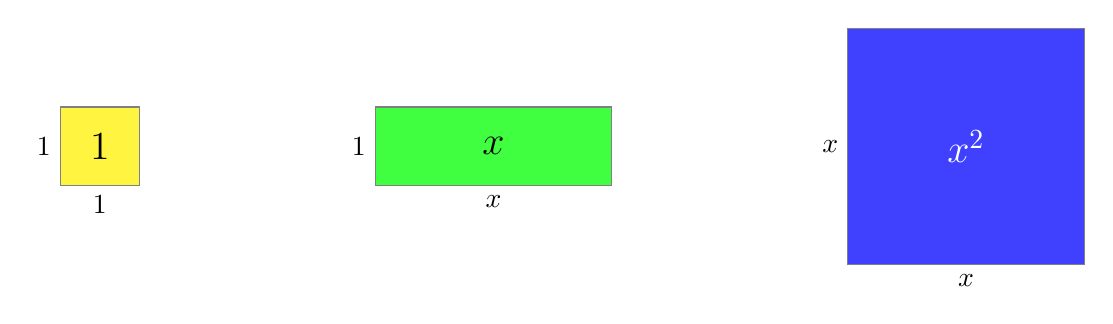
\begin{tikzpicture}
	%% 1 tile
	\draw[gray, fill=yellow!75] (0, 0) rectangle node[black]{\Large1} (1, 1);
	\draw (0.5, 0) node[below] {1};
	\draw (0, 0.5) node[left] {1};
	%% x tile
	\draw[gray, fill=green!75] (4, 0) rectangle node[black]{\Large$x$} (7, 1);
	\draw (5.5, 0) node[below] {$x$};
	\draw (4, 0.5) node[left] {1};
	%% xx tile
	\draw[gray, fill=blue!75] (10, -1) rectangle node[white]{\Large$x^2$} (13, 2);
	\draw (11.5, -1) node[below] {$x$};
	\draw (10, 0.5) node[left] {$x$};
\end{tikzpicture}
\end{center}

To multiply, say, $(x+4)^2$, we create a rectangle (a square, actually) that is ``x+4'' units on each side, and we fill in the area with our tiles.

\begin{center}
\begin{minipage}{0.48\textwidth}
\centering
\begin{tikzpicture}[scale=0.75]
	\draw[|-|] (0,0.1) -- node[above]{$x$} (3,0.1);
	\foreach \x in {3,...,6} {
		\draw[|-|] (\x,0.1) -- node[above]{1} (\x+1,0.1);
	}
	\draw[|-|] (-0.1,0) -- node[left]{$x$} (-0.1,-3);
	\foreach \y in {-3,...,-6} {
		\draw[|-|] (-0.1,\y) -- node[left]{1} (-0.1,\y-1);
	}
	\draw[gray] (0,0) rectangle (7,-7);
\end{tikzpicture}
\end{minipage}
\begin{minipage}{0.48\textwidth}
\centering
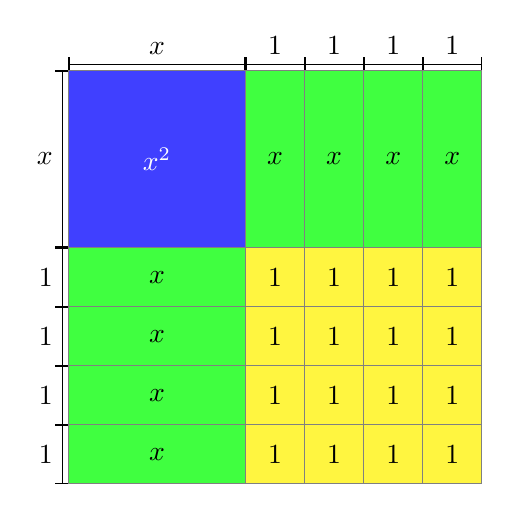
\begin{tikzpicture}[scale=0.75]
	\draw[|-|] (0,0.1) -- node[above]{$x$} (3,0.1);
	\draw[|-|] (-0.1,0) -- node[left]{$x$} (-0.1,-3);
	\draw[gray, fill=blue!75] (0,0) rectangle node[white]{$x^2$} (3,-3);
	\foreach \x in {3,...,6} {
		\draw[|-|] (\x,0.1) -- node[above]{1} (\x+1,0.1);
		\draw[gray, fill=green!75] (\x,0) rectangle node[black]{$x$} (\x+1,-3);
	}
	\foreach \y in {-3,...,-6} {
		\draw[|-|] (-0.1,\y) -- node[left]{1} (-0.1,\y-1);
		\draw[gray, fill=green!75] (0,\y) rectangle node[black]{$x$} (3,\y-1);
	}
	\foreach \x in {3,...,6} {
		\foreach \y in {-3,...,-6}
			\draw[gray, fill=yellow!75] (\x, \y) rectangle node[black]{1} (\x+1,\y-1);
	}
\end{tikzpicture}
\end{minipage}
\end{center}
The area is filled in with one $x^2$-tile, eight $x$-tiles, and sixteen 1-tiles. So, we have a total area of $x^2 + 8x + 16$.

\subsection{Beyond Squares}

Of course, the methods above all work for multiplying other expressions as well --- not just something times itself. Can you extend the models above to find the product of, say, \[(3x + 4)(2x + 3)\] When we multiply, we get the product $6x^2 + 17x + 12$. How can we get to this product using the ``double distribution'' approach? What about the old-school method? What would the algebra tiles area model look like?

We can also raise an expression to a power other than 2. For instance, we could raise an expression to the third power, as in the example below. There's a lot going on here, read through the work slowly and see if you can understand each step.
\[\begin{aligned}
(2x+5)^3 &= (2x+5)(2x+5)(2x+5)
\\
&= (4x^2+20x+25)(2x+5)
&&\quad\text{multiply the first two terms}
\\
&= 2x(4x^2+20x+25) + 5(4x^2+20x+25)
&&\quad\text{distribute the three-term expression!}
\\
&= \underline{8x^3 + 40x^2 + 50x} + \underline{20x^2 + 100x + 125}
&&\quad\text{distribute twice more}
\\
&= 8x^3 + 60x^2 + 150x + 125
&&\quad\text{combine like terms}
\end{aligned}\]
